\chapter{Exploratory Data Analysis}
\label{chapter_data_exploration}
%%%%%%%%%%%% FIGURE %%%%%%%%%%%
\newlength{\BoxPlotFigWidth} \setlength{\BoxPlotFigWidth}{0.48\textwidth}
\newlength{\BoxPlotFigHeight}
\settoheight{\BoxPlotFigHeight}{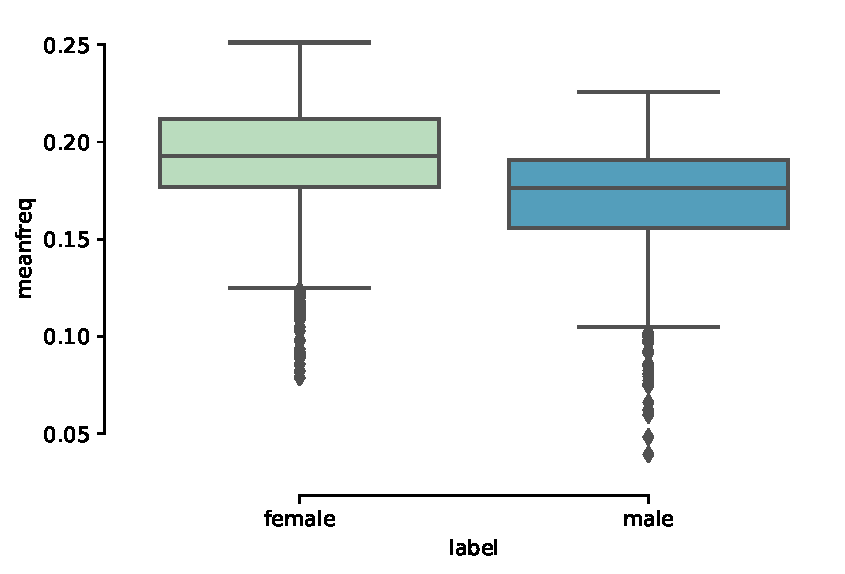
\includegraphics[width=\BoxPlotFigWidth]{figures/meanfreq_boxplot.pdf}}
\begin{figure}[htb]
	% Maximum length
	\hfill%
	\subcaptionbox{\label{fig_meanfreq_box}}{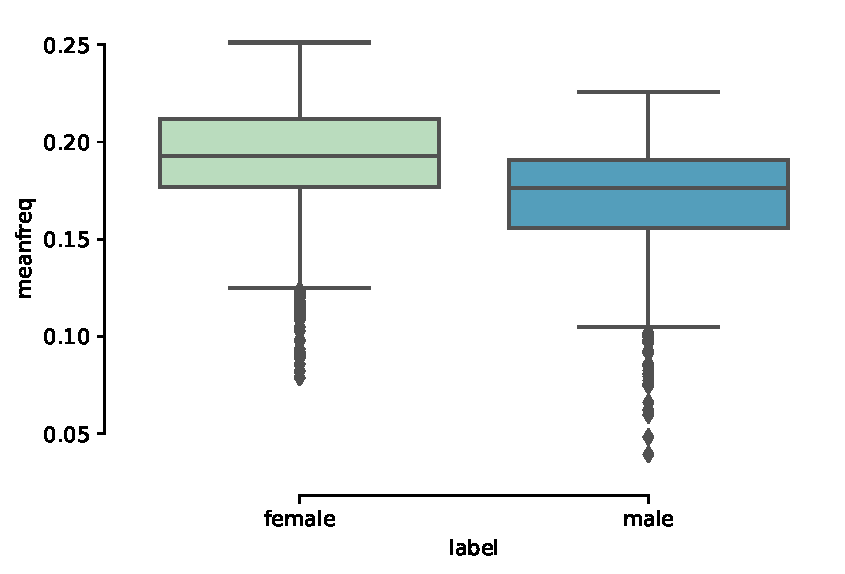
\includegraphics[height=\BoxPlotFigHeight]{figures/meanfreq_boxplot.pdf}}\hfill%
	\subcaptionbox{\label{fig_meanfun_box}}{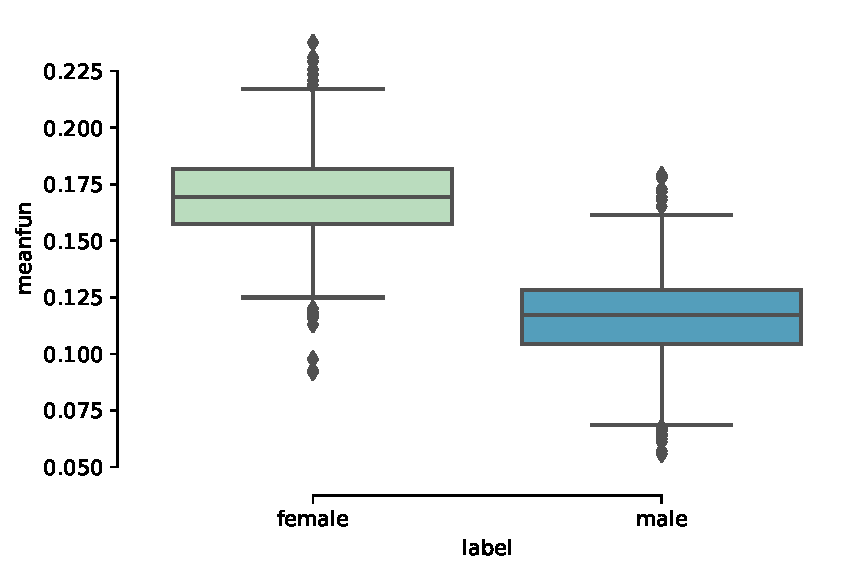
\includegraphics[height=\BoxPlotFigHeight]{figures/meanfun_boxplot.pdf}}\hfill\null%
	\caption{}
	\label{fig_mean_freq}
\end{figure}

\settoheight{\BoxPlotFigHeight}{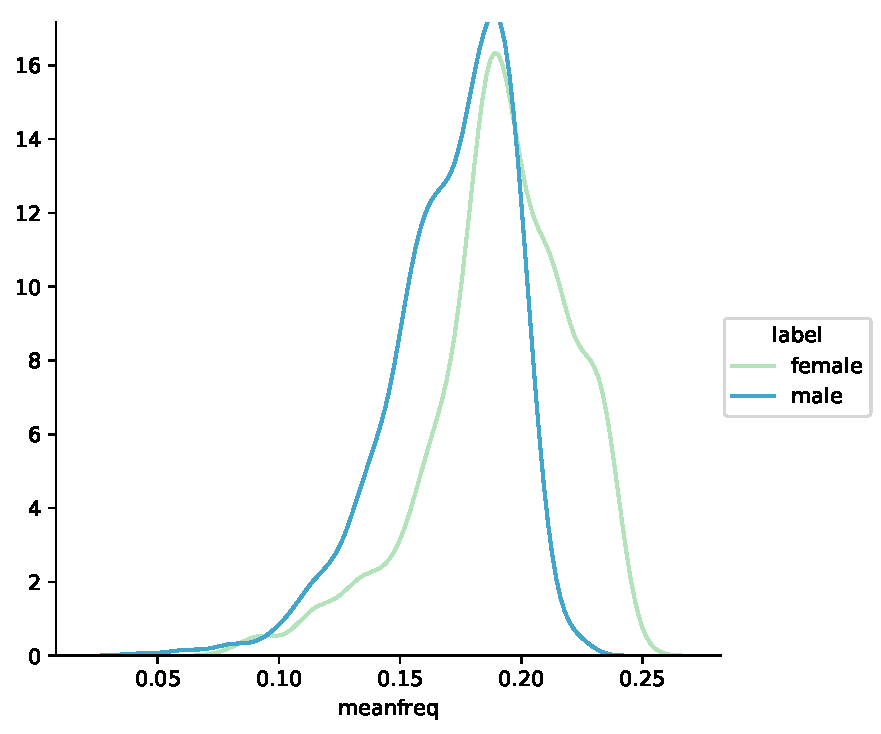
\includegraphics[width=\BoxPlotFigWidth]{figures/meanfreq_facetgrid.pdf}}
\begin{figure}[htb]
	% Maximum length
	\hfill%
	\subcaptionbox{\label{fig_meanfreq_facet}}{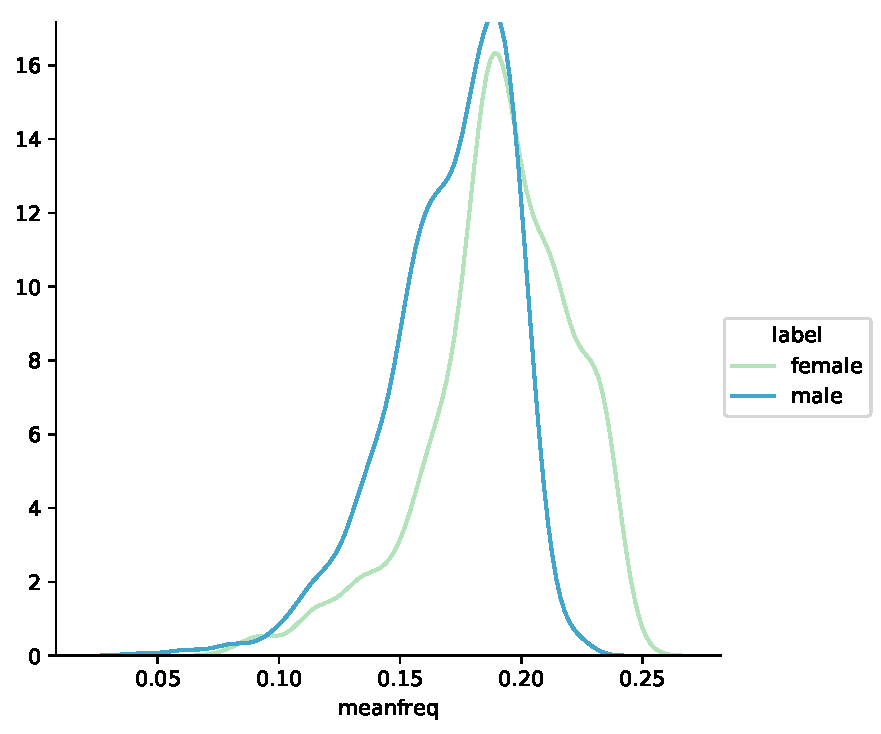
\includegraphics[height=\BoxPlotFigHeight]{figures/meanfreq_facetgrid.pdf}}\hfill%
	\subcaptionbox{\label{fig_meanfun_facet}}{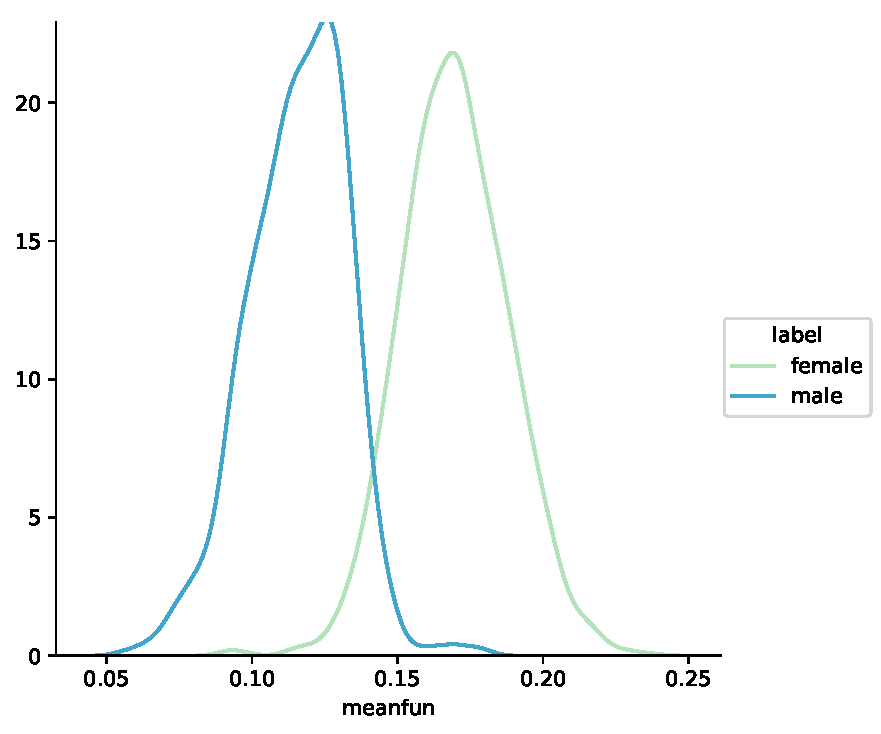
\includegraphics[height=\BoxPlotFigHeight]{figures/meanfun_facetgrid.pdf}}\hfill\null%
	\caption{}
	\label{fig_facet}
\end{figure}

\setlength{\BoxPlotFigWidth}{\textwidth}
\settoheight{\BoxPlotFigHeight}{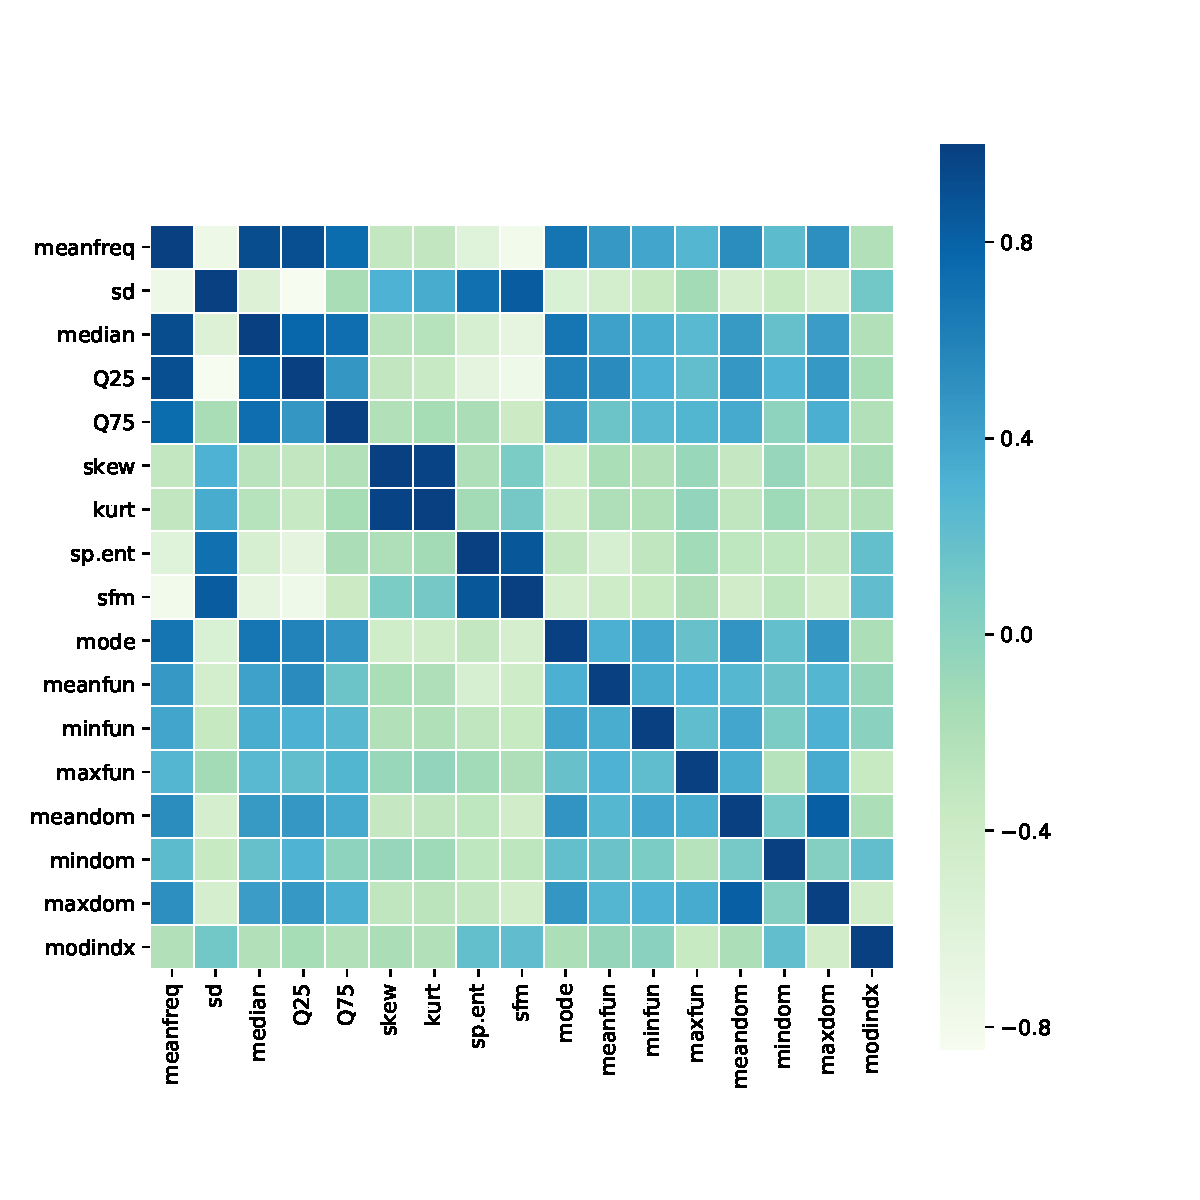
\includegraphics[width=\BoxPlotFigWidth]{figures/correlation_matrix.pdf}}
\begin{figure}[htb]
	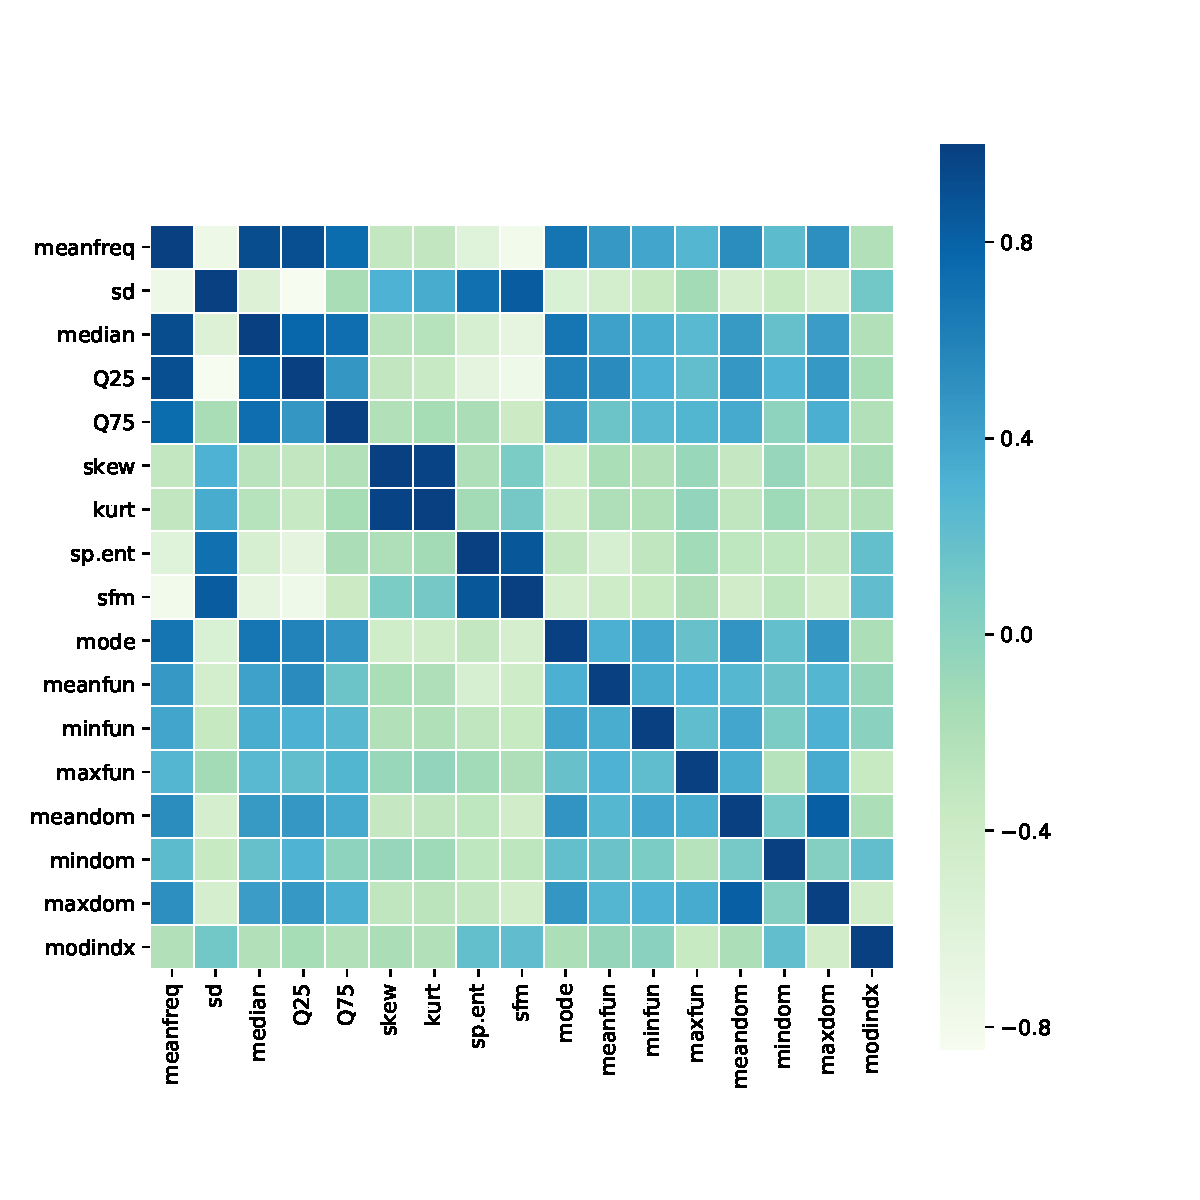
\includegraphics[height=\BoxPlotFigHeight]{figures/correlation_matrix.pdf}
	\caption{}
	\label{fig_corr_matrix}
\end{figure}
